% Created 2022-09-26 Mon 09:57
\documentclass[9pt, b5paper]{article}
\usepackage{xeCJK}
\usepackage{minted}
\usepackage[T1]{fontenc}
\usepackage[scaled]{beraserif}
\usepackage[scaled]{berasans}
\usepackage[scaled]{beramono}
\usepackage{graphicx}
\usepackage{xcolor}
\usepackage{multirow}
\usepackage{multicol}
\usepackage{float}
\usepackage{textcomp}
\usepackage{algorithm}
\usepackage{algorithmic}
\usepackage{latexsym}
\usepackage{natbib}
\usepackage{geometry}
\geometry{left=1.2cm,right=1.2cm,top=1.5cm,bottom=1.2cm}
\newminted{common-lisp}{fontsize=\footnotesize} 
\usepackage[xetex,colorlinks=true,CJKbookmarks=true,linkcolor=blue,urlcolor=blue,menucolor=blue]{hyperref}
\author{deepwaterooo}
\date{\today}
\title{Unity Android SDK/NDK 俄罗斯方块砖3D 小游戏}
\hypersetup{
  pdfkeywords={},
  pdfsubject={},
  pdfcreator={Emacs 27.1 (Org mode 8.2.7c)}}
\begin{document}

\maketitle
\tableofcontents


\section{模块搭建}
\label{sec-1}
\begin{itemize}
\item ILRuntime的消化理解,以及与MVVM同用时的搭配理解消化
\item 热更新模块服务器模块的理解与消化搭建:
\end{itemize}

\section{把原理弄懂}
\label{sec-2}
\begin{itemize}
\item 热更新模块的实充:以前的设计模式和实现的功能还是比较完整的;现在更成熟一点儿,需要把热更新模块补充出来;
\item ILRuntime + MVVM框架设计:两者结合,前几年的时候没能把MVVM理解透彻;
\item 上次前几年主要的难点:好像是在把MVVM双向数据绑定理解得不透彻;那么这次应该就狠没有问题了,更该寻求更好的设计与解决方案
\item 性能优化:另外是对其实高级开发的越来越熟悉,希望应用的性能表现,尤其是渲染性能与速度等、这些更为高级和深入的特性成为这次二次开发的重点。

\item 现在是把自己几年前的写的游戏全忘记了,需要回去把自己的源码找出来,再读一读熟悉一下自己的源码,了解当时设计的估缺点,由此改进更将
\end{itemize}

\section{环境弄得比较好的包括:}
\label{sec-3}
\begin{itemize}
\item 输入法的搭建:终于用到了自己之前用过的好用的输入法
\end{itemize}

\section{ILRuntime 库的系统再深入理解}
\label{sec-4}
\subsection{ILRuntime基本原理\#}
\label{sec-4-1}
\begin{itemize}
\item ILRuntime借助Mono.Cecil库来读取DLL的PE信息,以及当中类型的所有信息,最终得到方法的IL汇编码,然后通过内置的IL解译执行虚拟机来执行DLL中的代码。IL解释器代码在ILIntepreter.cs,通过Opcode来逐语句执行机器码,解释器的代码有四千多行。
\end{itemize}

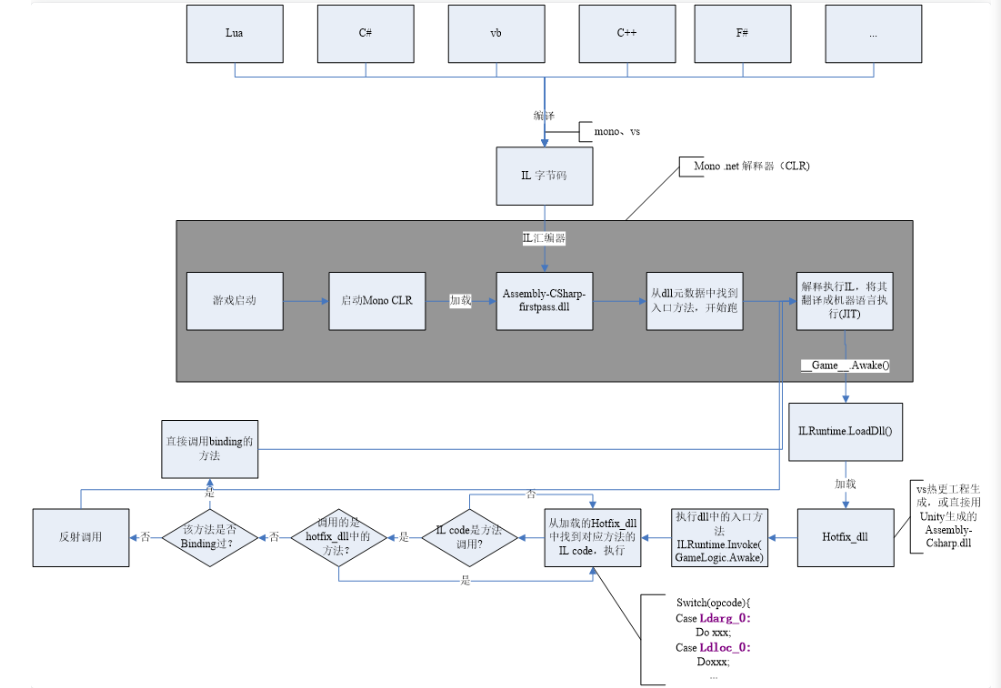
\includegraphics[width=.9\linewidth]{./pic/readme_20220926_094936.png}
\subsection{ILRuntime热更流程}
\label{sec-4-2}

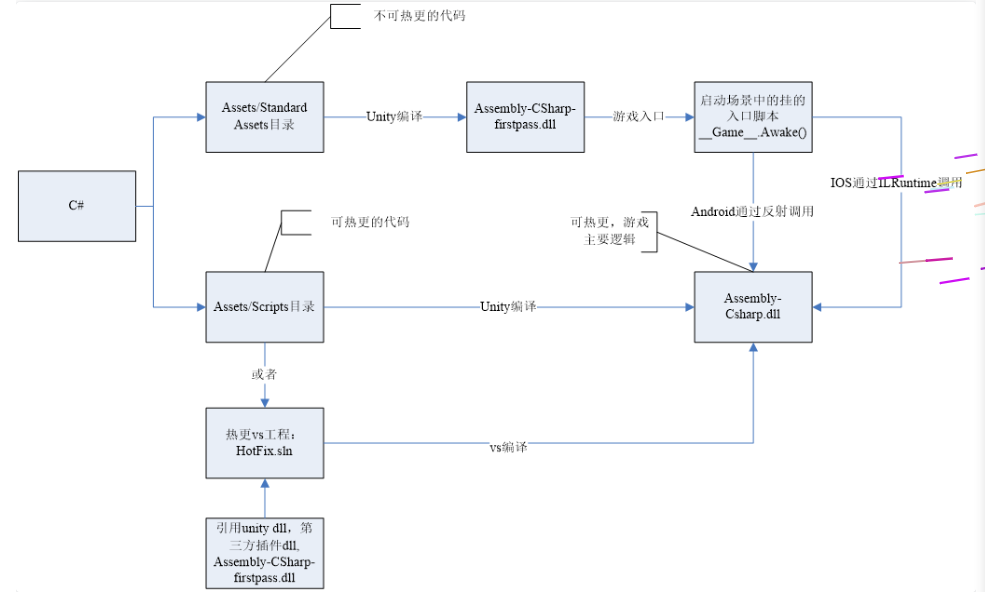
\includegraphics[width=.9\linewidth]{./pic/readme_20220926_095022.png}
\subsection{ILRuntime主要限制}
\label{sec-4-3}

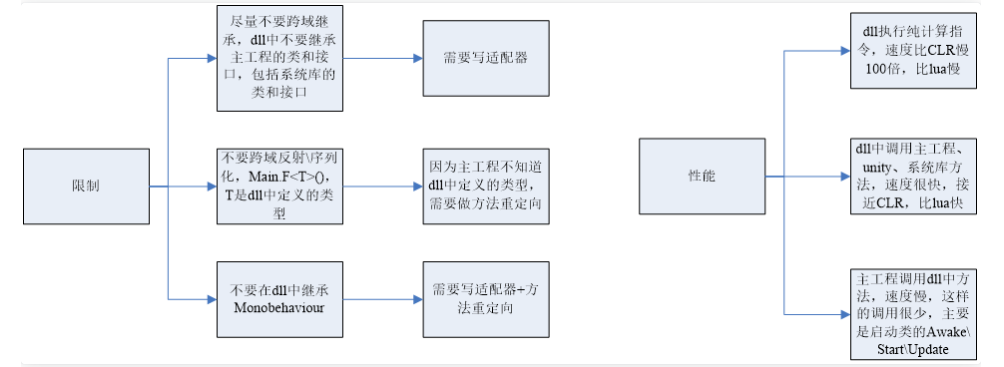
\includegraphics[width=.9\linewidth]{./pic/readme_20220926_095555.png}
\subsection{ILRuntime启动调试\#}
\label{sec-4-4}
\begin{itemize}
\item ILRuntime建议全局只创建一个AppDomain,在函数入口添加代码启动调试服务
\end{itemize}
\begin{minted}[fontsize=\scriptsize,linenos=false]{csharp}
appdomain.DebugService.StartDebugService(56000)
\end{minted}
\begin{itemize}
\item 运行主工程(Unity工程)
\item 在热更的VS工程中 点击 - 调试 - 附加到ILRuntime调试,注意使用一样的端口
\item 如果使用VS2015的话需要Visual Studio 2015 Update3以上版本
\end{itemize}
\subsection{线上项目和资料\#}
\label{sec-4-5}
\begin{itemize}
\item 掌趣很多项目都是使用ILRuntime开发,并上线运营,比如:真红之刃,境·界 灵压对决,全民奇迹2,龙族世界,热血足球
\item 初音未来:梦幻歌姬 使用补丁方式:\url{https://github.com/wuxiongbin/XIL}
\item 本文流程图摘自:ILRuntime的QQ群的《ILRuntime热更框架.docx》(by a 704757217)
\item Unity实现c\#热更新方案探究(三): \url{https://zhuanlan.zhihu.com/p/37375372}
\end{itemize}
% Emacs 27.1 (Org mode 8.2.7c)
\end{document}